%\pagenumbering{arabic}

\section{Memory Management}
\subsection{Physical Page Management}
\subsubsection{Homework \Rmnum{3}}
\begin{flushleft}
{\Large Question}
\end{flushleft}

In the file kern/pmap.c, you need to implement the code for the following function (see below, given in order):

Boot\_alloc()

Mem\_init() (before calling check\_page\_free\_list(1))

Page\_init()

Page\_alloc()

Page\_free()

Check\_page\_free\_list() and check\_page\_alloc() will test your physical page allocator. You need to guide JOS

Then check the success report for check\_page\_alloc(). It would be helpful to add your own assert() to verify that your assumptions are correct.
\begin{flushleft}
{\Large Theoretical preparation}
\end{flushleft}


The operating system must keep track of which memory regions are free and which are occupied. The JOS kernel manages memory with the minimum granularity of pages (pages), which uses the MMU to map and protect the memory allocated for each block.

Here we have to write the allocation subfunction of the physical memory page. It uses a linked list of structure PageInfo to record which pages are free, and each node in the linked list corresponds to a physical page.

\begin{flushleft}
{\Large Analysis \& Answer}
\end{flushleft}

The operating system must keep track of which physical RAM is free and which is in use. This exercise mainly writes a physical page allocator. It uses a linked list of PageInfo structures to record which pages are free, and each structure corresponds to a physical page.

Because the implementation of the page table requires the allocation of physical memory to store the page table, we need to write the physical page allocator before the implementation of the virtual memory.
\begin{figure}[H]
\centering
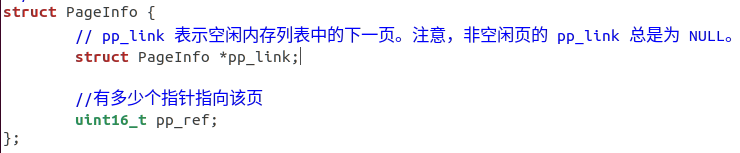
\includegraphics[width=0.8\linewidth]{figure/PageInfo}
\caption{Definition of PageInfo in memlayout.h}
\end{figure}


In the file kern/pmap.c, the function mem\_init() is called when the kernel first starts running, and some initialization settings are made for the memory management system of the entire operating system.

[Step 1] Enter mem\_init(). The first step is to call the sub-function i386\_detect\_memory() to check how much total memory space is available in the system and how much the three parts of the memory space are, and divide the page according to the set PGSIZE. The total number of pages and the number of pages in each of the three parts are calculated in the function.

JOS divides the entire physical memory space into three parts:

1 Basemen: Available from 0x00000 to 0xA0000

2 IO hole: From 0xA0000 to 0x100000, not available, mainly used to allocate to external devices.

3 Extmen: From 0x100000 to 0x, available, the most important memory area.

\begin{figure}[H]
\centering
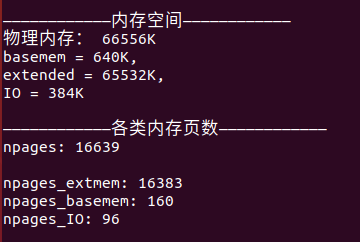
\includegraphics[width=0.8\linewidth]{figure/i386_detect_memory}
\caption{i386\_detect\_memory() run result}
\end{figure}

[Step 2] (1) Call the function boot\_alloc function to allocate a virtual memory of size PGSIZE followed by the operating system kernel bss for storing the operating system page table. When the operating system is working in virtual memory mode, this page directory table is required for address translation (virtual address→physical address).
The boot\_alloc function can be used to allocate virtual memory, and its parameter is the virtual memory byte size to be allocated. When 0 is input, the currently used virtual memory tail can be queried. The core idea of ​​this function is to maintain a static variable nextfree, which stores the virtual address corresponding to the next free memory space that can be used. The first time you enter the function you need to initialize nextfree. Note: The allocated memory size needs to be aligned with PGSIZE by the ROUNDUP function.

\begin{figure}[H]
\centering
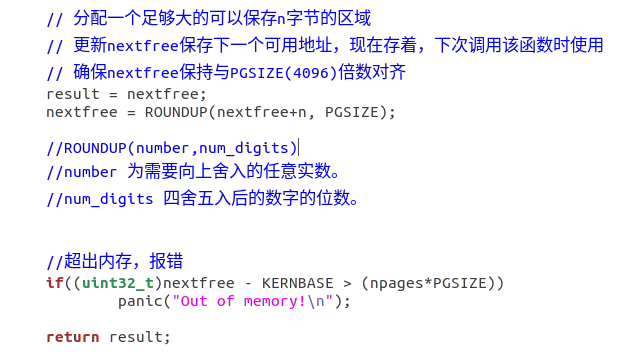
\includegraphics[width=0.8\linewidth]{figure/boot_alloc_changed}
\caption{The code supplemented by the boot\_alloc() function}
\end{figure}

(2) Initialize a pointer in physical memory kern\_pgdir points to the above operating system page table.

(3) Call the memset function to clear the virtual memory of the operating system page table area.

\begin{figure}[H]
\centering
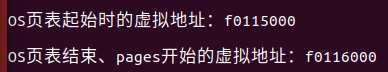
\includegraphics[width=0.8\linewidth]{figure/PGSIZE}
\caption{By information printing, the OS page table end address - OS page table start address = PGSIZE}
\end{figure}


[Step 3] Add the first page directory entry for the page directory table just created, occupying the 0th position of the page table. The content of the entry is the real address of the pointer kern\_pgdir. UVPT is defined as the starting address of a virtual address, 0xef400000. Starting from this virtual address, the page table kern\_pgdir of this operating system is stored, so we must map it to the physical address of the page table kern\_pgdir, PADDR(kern\_pgdir) It is calculating the real physical address corresponding to kern\_pgdir.
\begin{figure}[H]
\centering
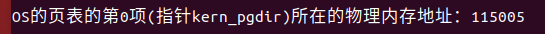
\includegraphics[width=0.8\linewidth]{figure/real_physical_address}
\caption{The actual physical address of the pointer is known by information printing.}
\end{figure}

[Step 4] Use the boot\_alloc function to allocate a virtual memory of size npages * sizeof(struct PageInfo), which is used to store an array of struct PageInfo. The pointers in memory point to the virtual memory. The OS uses this array to track the usage of all memory pages. Each PageInfo represents a page in memory. PageInfo has two attributes: 1. Whether the current page is occupied. 2. Pointer to the next page. Then call the memset function to clear the corresponding area memory.

\begin{figure}[H]
\centering
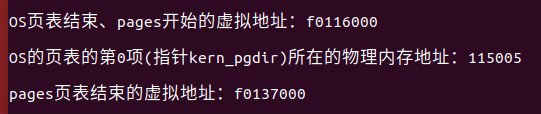
\includegraphics[width=0.8\linewidth]{figure/pages_alloc_virtualmem}
\caption{Allocate virtual memory for pages}
\end{figure}

Note: It is found through information printing that the memory address at the end of the pages page table minus the memory address at the beginning of the pages is not exactly equal to npages * sizeof(struct PageInfo), but slightly larger than when the virtual memory is allocated in the boot\_alloc function. It needs to be noted that it is aligned with the PGSIZE multiple, so the allocated virtual memory size is appropriately allocated upwards.

[Step 5] Call the function page\_init() to initialize the linked list of two struct pageinfo pages and page\_free\_list. The pages\_free\_list linked list stores all the free page information, and the pages store the information of the free\\non-free pages.

Jos divides the entire physical memory space into three parts, namely BASEMEM, IO HOLE, and EXTMEM.

According to the first item of the known basemem is already occupied, and other pages of basemem are not occupied. Since IO HOLE is mainly used to be allocated to external devices and is not available, it is equivalent to occupying all pages. EXTMEM is occupied in the first part of the page in step four, and part of it is idle.
\begin{figure}[H]
\centering
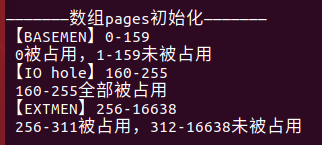
\includegraphics[width=0.8\linewidth]{figure/pages_init}
\caption{Pages initialization result}
\end{figure}

\begin{figure}[H]
\centering
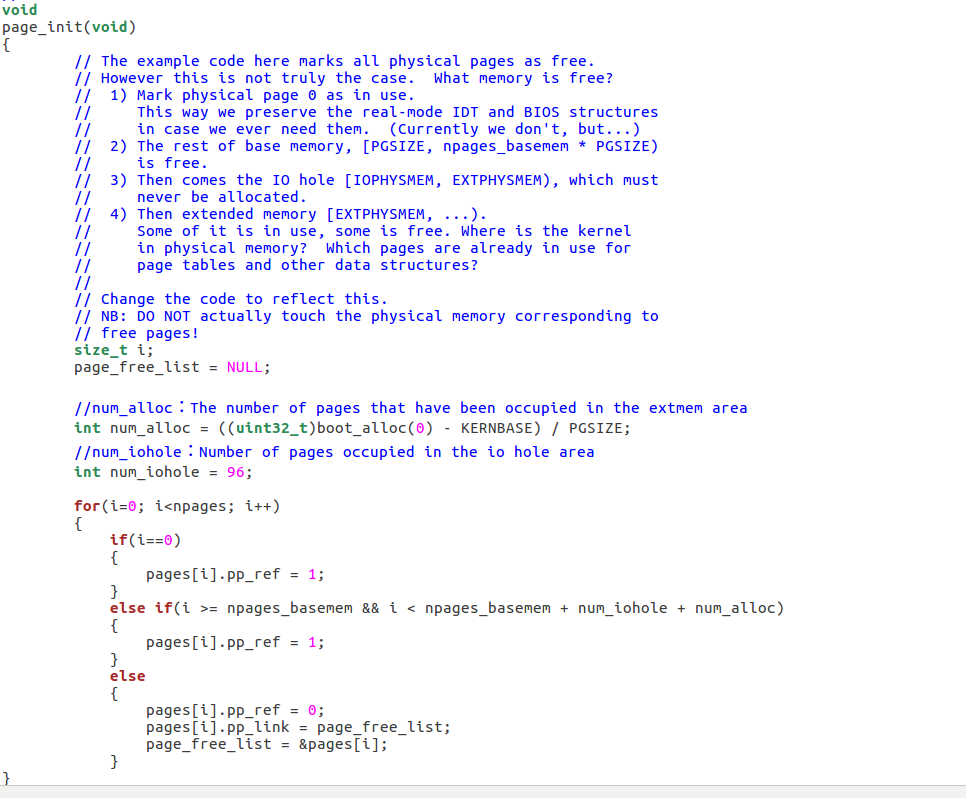
\includegraphics[width=0.8\linewidth]{figure/page_init_changed}
\caption{page\_init() supplemental code screenshot}
\end{figure}

[Step 6] Call check\_page\_free\_list() and check\_page\_alloc() to test the above physical page allocator.

Check\_page\_free\_list() checks whether the so-called free pages of the page\_free\_list linked list are really legal and free. When the input parameter is 1, this function needs to perform one additional operation before checking, and modify the free page list free\_page\_list. After page\_init, free\_page\_list has stored all the free page tables, but their order is according to the page table. The numbers are arranged from large to small. In the page directory table entry\_pgdir (not kern\_pgdir) used by the current operating system, the page table of the large number is not mapped, so we cannot operate this part of the page table. However, the small numbered page table, that is, from the page table 0 to the page table 1023, has been mapped, so this page table can be operated. Then check\_page\_free\_list(1) is to complete the PageInfo structure corresponding to this part of the page table to the front end of the free\_page\_list for the operating system to use now. The rest of the operation is to check the free\_page\_list.

The function of the check\_page\_alloc() function is to check if page\_alloc() and page\_free() functions correctly.

One of the job requirements is to implement the page\_alloc() function. By commenting we can know that the function of this function is to allocate a physical page. The return value of the function is the PageInfo structure corresponding to this physical page. So the general steps of this function should be:

1. Take a PageInfo structure of a free page from free\_page\_list

2. Modify the free\_page\_list related information, such as modifying the linked list header

3. Modify the PageInfo structure information of the taken free page to initialize the memory of the page.

\begin{figure}[H]
\centering
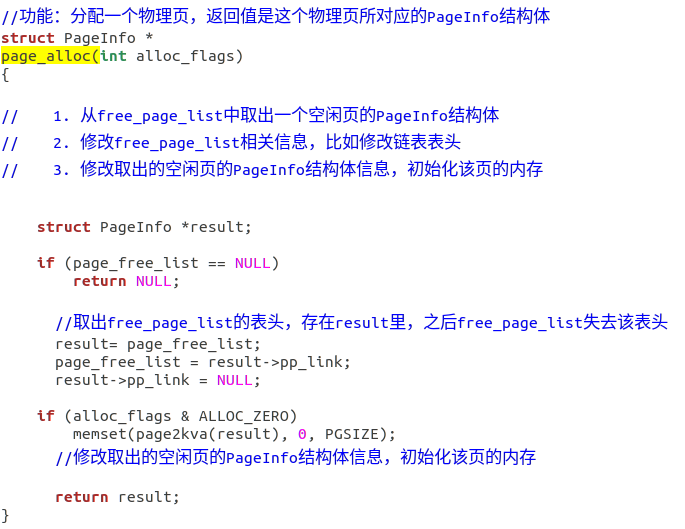
\includegraphics[width=0.8\linewidth]{figure/page_alloc_changed}
\caption{Page\_alloc() function complement code}
\end{figure}

Similarly, the job requires page\_free(). According to the comment, the function of this method is to return the PageInfo structure of a page to the page\_free\_list free page list, which means that the page is recycled. Mainly complete the following operations:

1. Modify the corresponding information of the PageInfo structure of the page being recycled.

2. Insert the structure back into the page\_free\_list free page list
\begin{figure}[H]
\centering
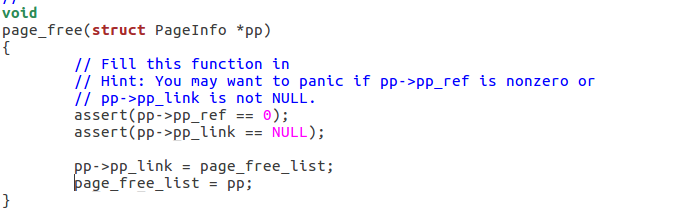
\includegraphics[width=0.8\linewidth]{figure/page_free_changed}
\caption{Page\_free function supplement code}
\end{figure}
\subsection{Virtual Memory}
\subsubsection{Exercise \Rmnum{4}}
\begin{flushleft}
{\Large Question}
\end{flushleft}

Read Chapters 5 and 6 of the Intel 80386 Reference Manual for reading about page conversion and page-based protection(5.2 and 6.4). We recommend that you briefly understand the chapter on segmentation mode, because although the use of JOS is based on
Page memory for virtual memory and protection, but segment conversion and segment-based protection cannot be disabled on x86, so you need
Have a basic understanding..

\begin{flushleft}
{\Large Answer}
\end{flushleft}

The logical address of the page consists of the page number and the in-page address

The physical address of the page is spliced ​​by the block number and the address within the page.

The purpose of the page table is to implement address mapping from page number to physical block number. The page table is retrieved by the page number of the logical address to obtain the physical block number of the page; and the in-page address d is directly sent into the block address field of the physical address register. In this way, the physical block number and the intra-block address are spliced ​​into an address that actually accesses the memory, thereby completing the conversion from the logical address to the physical address.

So the calculation formula for the physical address is:

Physical address = block size (ie page size L) ́ block number f + page address d

\subsubsection{Virtual address, linear address and physical address}

In the x86 architecture, a virtual address is composed of two parts, one is a segment selector and the other is a segment offset. A Linear Address refers to an address obtained by converting a virtual address by a segment address translation mechanism. A physical address (Physical Addresses) is the real memory address obtained by the paging address translation mechanism after converting the linear address. This address will eventually be sent to the address bus of your memory chip. The specific relationship of the three addresses is as follows
\begin{figure}[H]
\centering
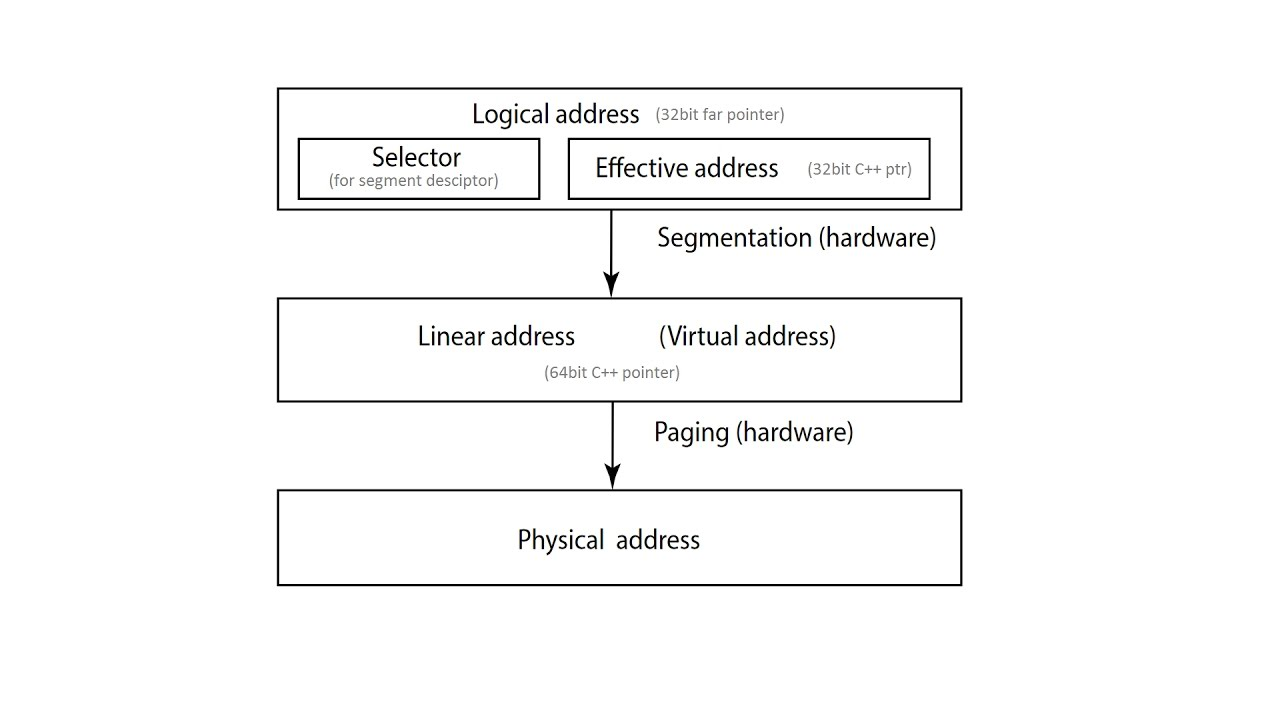
\includegraphics[width=0.8\linewidth]{figure/virtual_linear_physical_address}
\end{figure}

\subsubsection{Exercise \Rmnum{5}}
\begin{flushleft}
{\Large Question}
\end{flushleft}

GDB can only access QEMU's memory through virtual addresses, but when learning to create virtual addresses, we also need to check the physical address at the same time. Learn QEMU's monitor command, especially the xp command, which allows you to check physical memory.

\begin{flushleft}
{\Large Answer}
\end{flushleft}

Open Terminal, enter qemu-system-i386 -hda obj/kern/kernel.img -monitor stdio -gdb tcp::26000 -D qemu.log , after the correct installation, we can use the monitor command.
\begin{figure}[H]
\centering
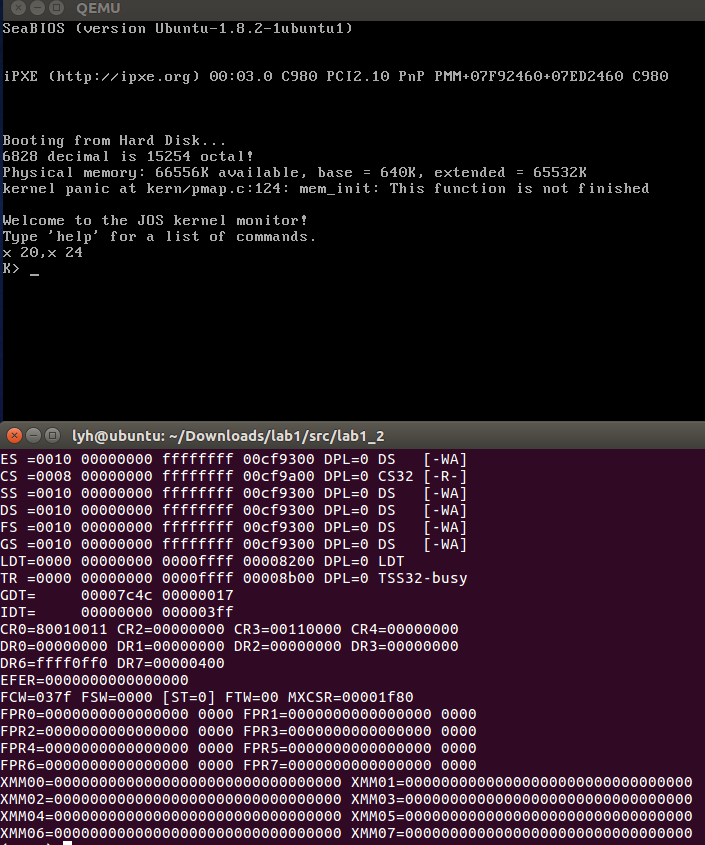
\includegraphics[width=0.8\linewidth]{figure/qemu_commond}
\caption{qemu command}
\end{figure}

\subsubsection{Question \Rmnum{3}}
\begin{flushleft}
{\Large Question}
\end{flushleft}

Assuming the following kernel code is correct, then what type of variable x will be, uintptr\_t or
Physaddr\_t?
\begin{flushleft}
Mystery\_t x;\\
Char* value = return\_a\_pointer();\\
*value = 10; \\
x =(mystery\_t) value;\\
\end{flushleft}
\begin{flushleft}
{\Large Answer}
\end{flushleft}

Since the * operator is used here to resolve the address, the variable x should be of type uintptr\_t.

\subsubsection{Reference counting}
In the previous experiment, we encountered pp\_ref, which records how many different virtual addresses exist on each physical page to reference it. When this value becomes 0, the physical page can be released. In general, the pp\_ref value of any physical page p is equal to the number of times it is mapped by the virtual page under the virtual address UTOP in all page table entries (the address range above UTOP is already mapped at startup) Finished, will not be changed afterwards).

\subsubsection{Page Table Management}
Now we can start writing programs that manage page tables: including inserting and deleting linear address-to-physical address mappings, and creating page tables.

\subsubsection{Homework \Rmnum{4}}
\begin{flushleft}
{\Large Question}\\
In the file kern/pmap.c, you must implement code for the following functions.\\
pgdir\_walk()\\
boot\_map\_region()\\
page\_lookup()\\
page\_remove()\\
page\_insert()\\	
check\_page(), called from mem\_init(), tests your page table management routines. You should make sure it reports success before proceeding.\\
\end{flushleft}
\begin{flushleft}
{\Large Theoretical preparation}
\end{flushleft}

In the previous description, we have a basic understanding of the concept of virtual address, linear address, and physical address.

{\large Physical address}

The unit addressing for the memory chip level corresponds to the address bus to which the processor and the CPU are connected.
- This concept should be the best understood of these concepts. However, it is worth mentioning that although the physical address can be directly understood as the memory itself inserted in the machine, the memory is treated as a large array of numbers from 0 bytes up to the maximum amount of bytes, and then this is An array is called a physical address. However, in fact, this is just an abstraction provided by the hardware to the software. The way memory is addressed is not the case. So, to say that it is "corresponding to the address bus" is more appropriate. Just aside from the consideration of the physical memory addressing mode, it is acceptable to directly compare the physical address with the physical memory. Perhaps the wrong understanding is more conducive to metaphysical abstraction.

{\large Virtual memory}

This is a description of the abstraction of the entire memory (not to the top of the machine).

It is relative to physical memory and can be directly understood as "not straight" and "fake" memory. For example, a 0x08000000 memory address. It is not correct for the address element of 0x08000000 -1 in the large array on the physical address.

The reason is this. Because modern operating systems provide a kind of memory management, that is, virtual memory. The process uses the address in virtual memory, which is assisted by the operating system to "convert" it into a real physical address.

This "conversion". It is the key to all issues discussed.
With this kind of abstraction. A program can use a much larger address space than the real physical address.

Even multiple processes can use the same address. Not surprisingly. Since the converted physical address is not the same.
—— Can decompile the connected program and find that the connector has assigned an address to the program. For example, to call a function A, the code is not call A, but call 0x0811111111, that is, function A The address has been fixed. Without such a "conversion", there is no concept of a virtual address, and doing so is simply not feasible.

{\large Logical address}

In order to be compatible, Intel has retained the segmental memory management method of ancient times.

A logical address is an address used in a machine language instruction to specify an operand or an instruction. In the above example, we say that the address assigned to A by the connector 0x08111111 is the logical address. . "A logical address is an offset of a segment identifier plus a relative address within a specified segment. It is expressed as [segment identifier: offset within segment], that is, the 0x08111111 in the above example should indicate For [A's code segment identifier: 0x08111111], this is complete."

{\large Linear address or virtual address (virtual address)}

Similar to the logical address, it is also an unreal address. If the logical address is the corresponding hardware platform segment management pre-conversion address, then the linear address corresponds to the pre-conversion address of the hardware page memory.

We also need to know the knowledge about the page table.

Our physical memory has a total of 4GB, and we assign it to the page, each page is 4KB in size.

The 4GB (2 to the 32th power) linear address space can be divided into 1048576 (2 to the 20th power, that is, 1M, can also be regarded as 1024 * 1024) pages, so you can randomly extract these pages, every 1024 The pages are a group and can be divided into 1024 groups. For each group of 1024 pages of physical addresses, arranged in a certain order can constitute a table (each entry is the physical address of a page), this table is the page table. The size of the page table is 1024*4B=4KB, which is exactly the size of a physical page.

Because it has been divided into 1024 groups, each group has a page table (size 4KB), so these 1024 page tables can be pointed to by a table, this is the page directory. Similar to the page table, the page directory has a total of 1024 entries (called page directory entries), and the content of each page directory entry is the physical address of a page table. The size of the page table is 1024*4B=4KB, which is exactly the size of a physical page.

The conversion of three addresses and the page table mechanism are shown in the figure below.
\begin{figure}[H]
\centering
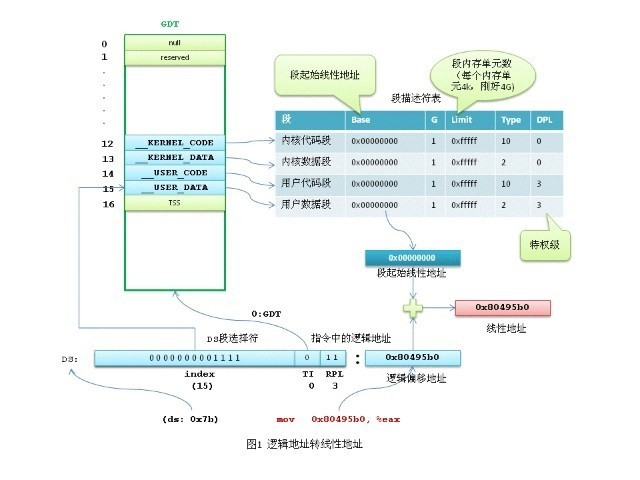
\includegraphics[width=0.8\linewidth]{figure/address_transform_1}
\end{figure}

\begin{figure}[H]
\centering
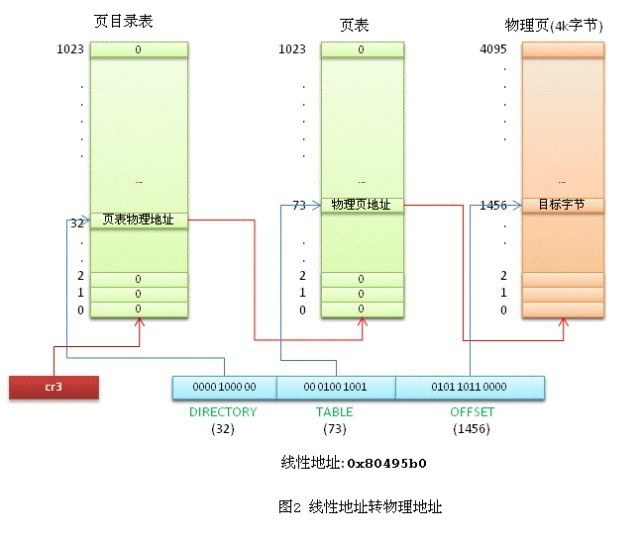
\includegraphics[width=0.8\linewidth]{figure/address_transform_2}
\end{figure}

\begin{figure}[H]
\centering
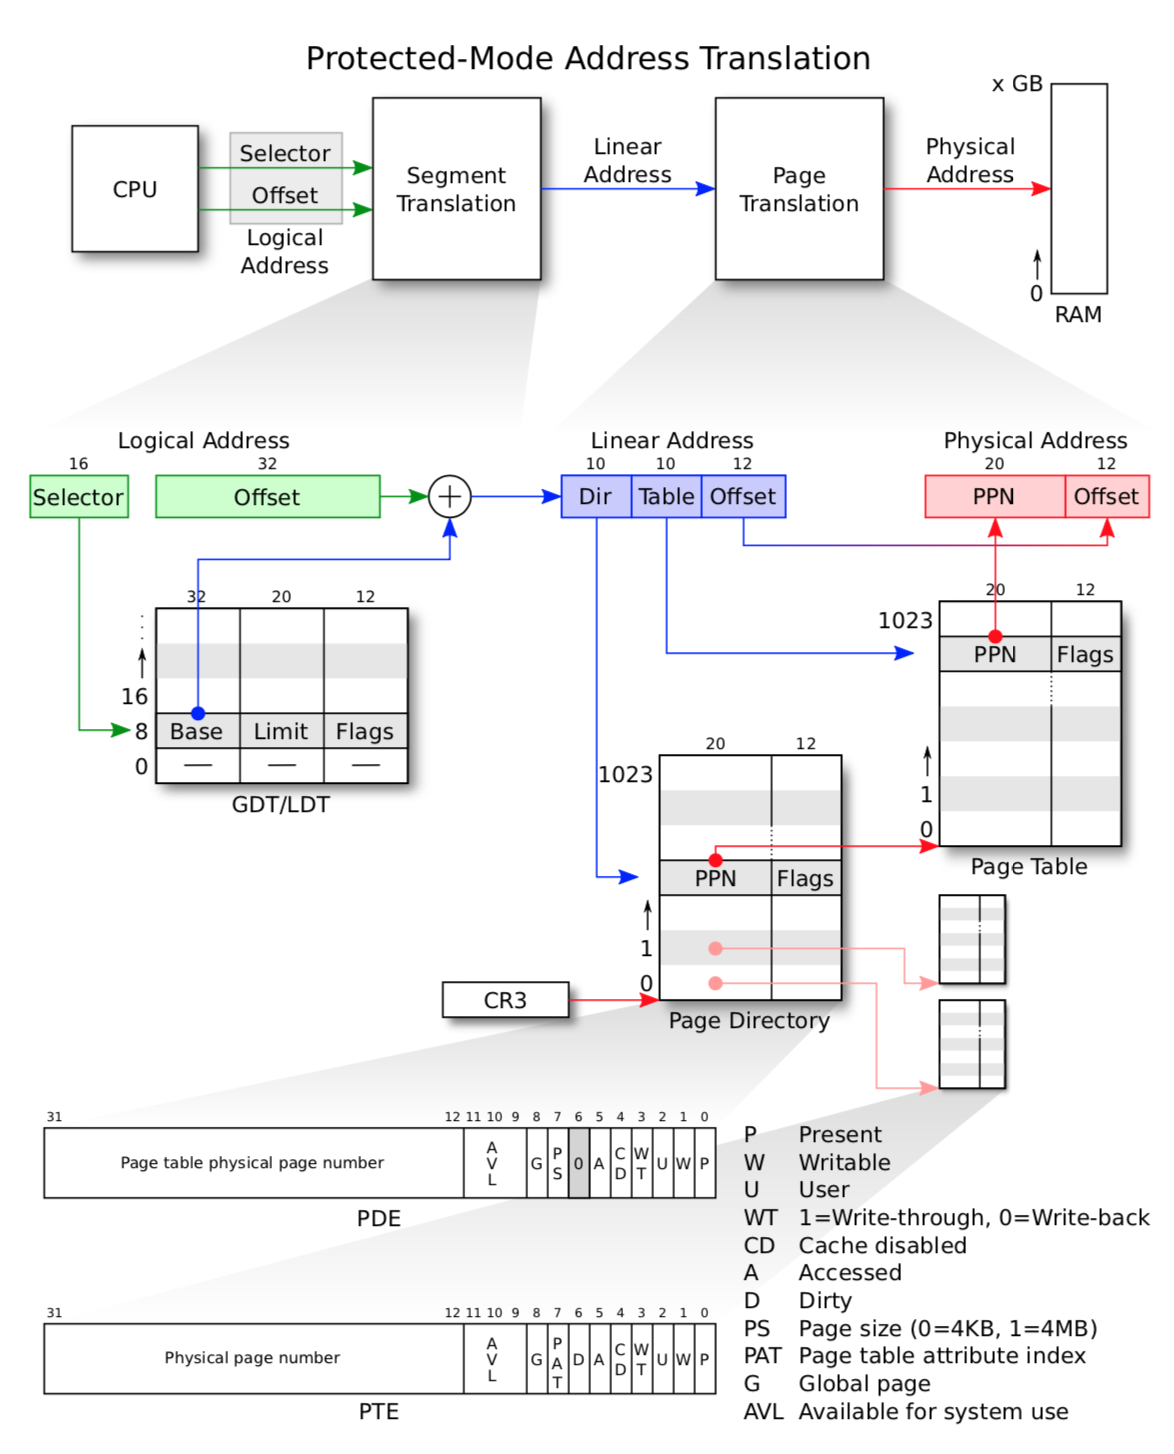
\includegraphics[width=0.8\linewidth]{figure/address_transform}
\end{figure}

\begin{flushleft}
{\Large Analysis \& Answer}
\end{flushleft}

By commenting, we can know that the function of this function is given a page directory table pointer pgdir , which should return the page table entry pointer corresponding to the linear address va.We need to complete the transformation as shown in the figure, return the corresponding page table address, that is, the virtual address of the part circled by the red circle:
\begin{figure}[H]
\centering
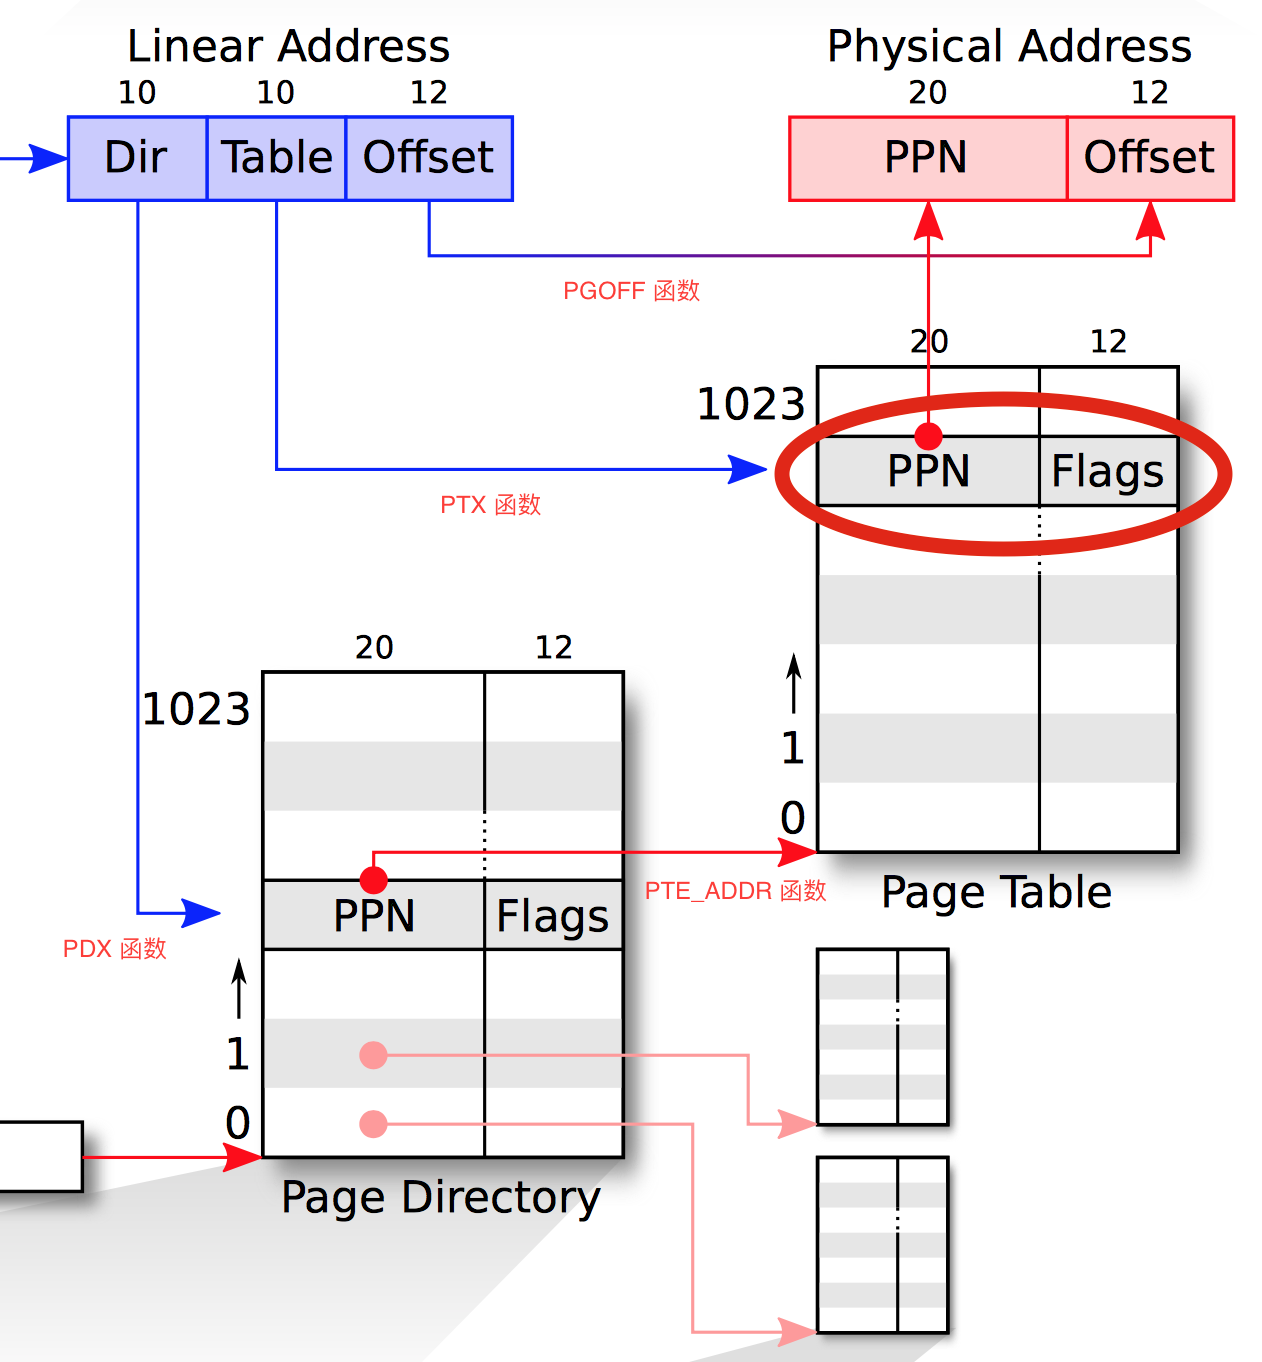
\includegraphics[width=0.8\linewidth]{figure/pgdir_walk_purpose}
\end{figure}

In addition, we need to understand the meaning of the three parameters.In addition, we need to understand the meaning of the three parameters, pgdir means the page directory item pointer, va means linear address, JOS equals virtual address, create means if page directory entry does not exist or not.

Here we should complete the following steps:

1. Find the page table page where the virtual address is located by the page directory table for the page directory entry address dic\_entry\_ptr in the page directory. (7-8)

2. Determine if the page table page corresponding to this page directory entry is already in memory. (10)

3. If yes, calculate the base address page\_base of this page table page, and then return the address of the page entry corresponding to va \&page\_base[page\_off] (23-25)

4. If not, and create is true, a new page is allocated, and the information of this page is added to the page directory entry dic\_entry\_ptr. (11-18)

5. If create is false, it returns NULL. (19-20)

The modified code is shown in the figure
\begin{figure}[H]
\centering
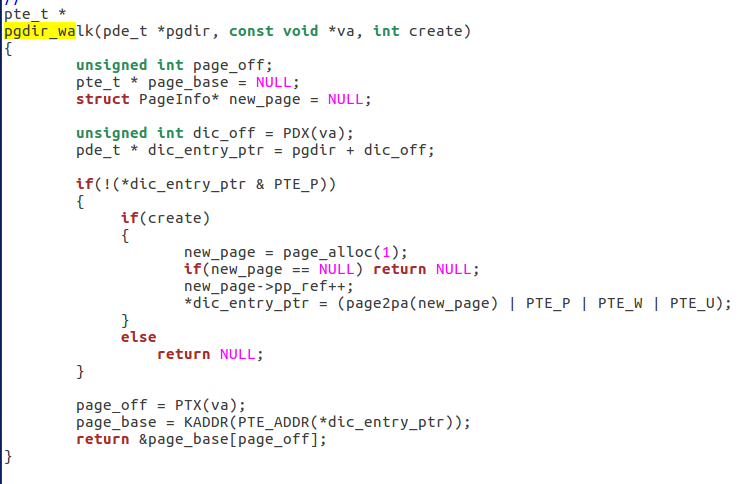
\includegraphics[width=0.8\linewidth]{figure/pgdir_walk_changed}
\caption{pgdir\_walk}
\end{figure}

Next we complete the boot\_map\_region function. By comment, we can see that the function of this function is to map [va, va+size) of virtual address space to physical [pa, pa+size) in the page table rooted at pgdir.  Size is a multiple of PGSIZE,and va and pa are both page-aligned.Use permission bits perm|PTE\_P for the entries.


The mapping of the virtual address space range [va, va+size) to the physical space [pa, pa+size) is added to the page table pgdir. The main purpose of this function is to set the address range above the virtual address UTOP. The address mapping of this part is static and will not change during the operation of the operating system, so the value of the pp\_ref field in the PageInfo structure of this page. No change will happen.

The steps to be completed by this function are as follows:

Need to complete a loop, using the pgdir\_walk function we just completed, we can use a loop to map all the memory in size bytes.The modified code is shown in the figure:
\begin{figure}[H]
\centering
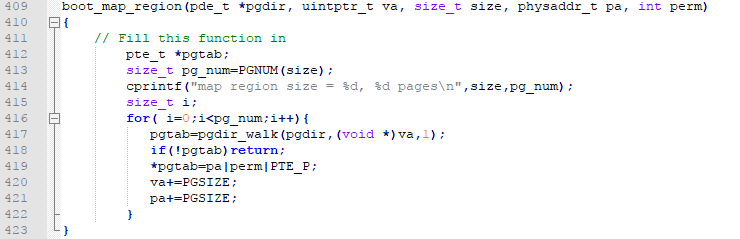
\includegraphics[width=0.8\linewidth]{figure/boot_map_region_changed}
\caption{boot\_map\_region}
\end{figure}

Next, continue to view page\_insert(). The function prototype is as follows: page\_insert(pde\_t *pgdir, struct PageInfo *pp, void *va, int perm), which is functionally completed: mapping a page pp in a physical memory to a virtual address va .

The main steps of this function are as follows:

1. First, find the page table entry corresponding to the virtual address va by using the pgdir\_walk function. (4)

2. Modify the value of pp\_ref. (8)

3. Check the page table entry to determine if va has been mapped. If it is mapped, delete the mapping. (9-13)

4. Add the mapping between va and pp to the page table entry. (14-15)

\begin{figure}[H]
\centering
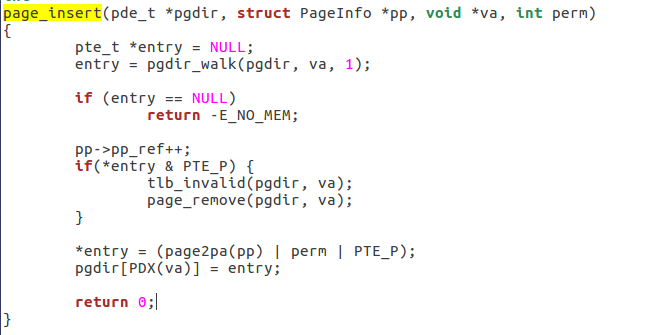
\includegraphics[width=0.8\linewidth]{figure/page_insert_changed}
\caption{page\_insert}
\end{figure}

Next, we complete the page\_lookup function, which functions as return the page mapped at virtual address 'va'.If the pte\_store parameter is not 0, the page table entry address of this physical page is stored in pte\_store.

We only need to call the pgdir\_walk function to get the page table entry corresponding to this va, and then determine whether the page is already in memory, and if so, return the PageInfo structure pointer of this page. And store the contents of this page table entry in pte\_store.The modified code is shown in the figure:
\begin{figure}[H]
\centering
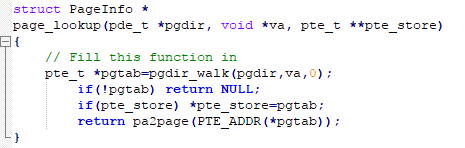
\includegraphics[width=0.8\linewidth]{figure/page_lookup_changed}
\caption{page\_lookup}
\end{figure}

The last one is the page\_remove function. Its prototype is: void page\_remove(pde\_t *pgdir, void *va). The function is to delete the mapping between the virtual address va and the physical page.

The note also hints at a few details to be aware of:

1. The pp\_ref value should be reduced by one.

2. If pp\_ref is reduced to 0, this page should be recycled

3. The page table entry corresponding to this page should be set to 0.

\begin{figure}[H]
\centering
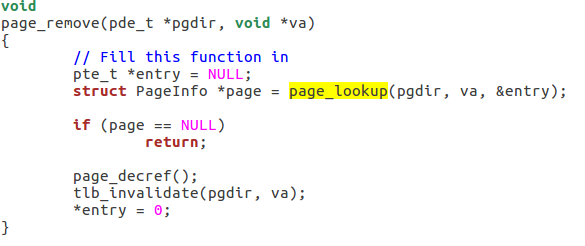
\includegraphics[width=0.8\linewidth]{figure/page_remove_changed}
\caption{page\_remove}
\end{figure}

\subsection{Kernel address space}

JOS divides the 32-bit linear address virtual space into two parts. The user environment (process running environment) usually occupies the part of the low address, called the user address space. The operating system kernel always occupies the part of the high address, called the kernel address space. The dividing line between these two parts is a macro ULIM defined in the memlayout.h file. JOS reserves nearly 256MB of virtual address space for the kernel. This can be understood, why in the experiment 1 to design a high address address space for the operating system. If you don't do this, the address space of the user environment is not enough.

\subsubsection{Homework \Rmnum{5}}
\begin{flushleft}
{\Large Question}
\end{flushleft}
Fill in the missing code in mem\_init() after the call to check\_page().

\begin{flushleft}
{\Large Theoretical preparation}
\end{flushleft}

Since the kernel and user memory are present in the address space of each environment, we need to use the permission bits in the x86 page table to allow the user code to access only the user portion of the address space. Otherwise, bugs in the user code may overwrite the kernel data, causing a crash; or the user code can steal private data from other environments.
The user environment will have no access to any memory above ULIM, and the kernel can read and write this portion of memory. For the address range [UTOP, ULIM), the kernel and the user environment have the same permissions: they can only be read and not written. Under UTOP
The address space is used by the user environment, and the user environment will set permissions to access this part of the memory.
\begin{figure}[H]
\centering
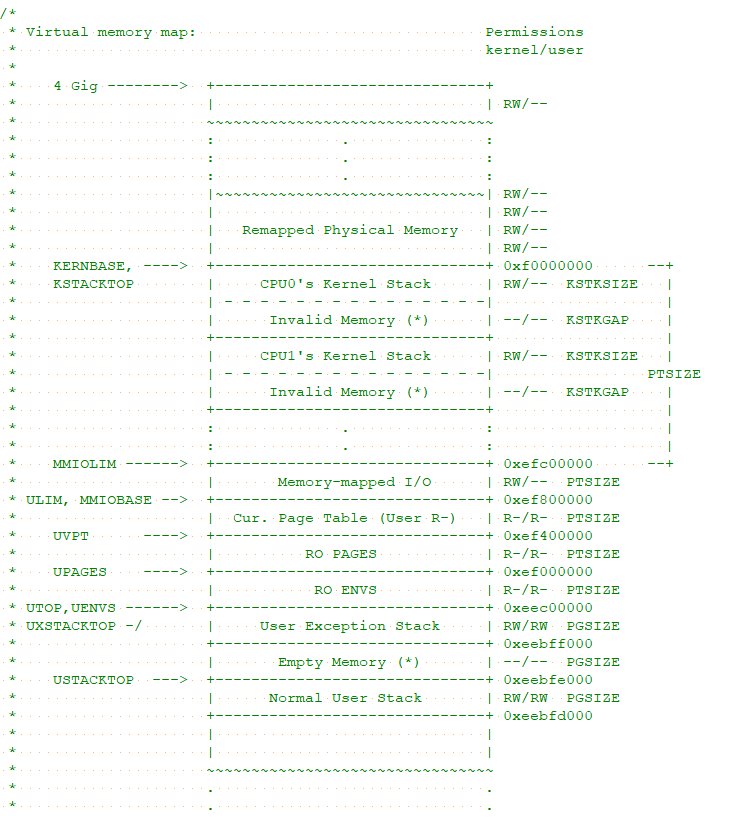
\includegraphics[width=0.8\linewidth]{figure/mem_layout}
\end{figure}

\begin{flushleft}
{\Large Analysis \&Answer}
\end{flushleft}

In this exercise, three virtual addresses are mapped to the physical page.

First, we will complete the UPAGES mapping UPAGES (0xef000000 \~ 0xef400000) up to 4MB, which is the data structure of JOS recording physical page usage.

Currently only one page directory is created, kernel\_pgdir, so the first parameter is obviously kernel\_pgdir. The second parameter is the virtual address, and UPAGES is originally given as a virtual address. The third parameter is the mapped memory block size. The fourth parameter is the physical address mapped to, and the physical address of pages can be taken directly. Permissions PTE\_U indicates that the user has permission to read.Currently only one page directory is created, kernel\_pgdir, so the first parameter is obviously kernel\_pgdir. The second parameter is the virtual address, and UPAGES is originally given as a virtual address. The third parameter is the mapped memory block size. The fourth parameter is the physical address mapped to, and the physical address of pages can be taken directly. Permissions PTE\_U indicates that the user has permission to read.
The modified code is shown in the figure
\begin{figure}[H]
\centering
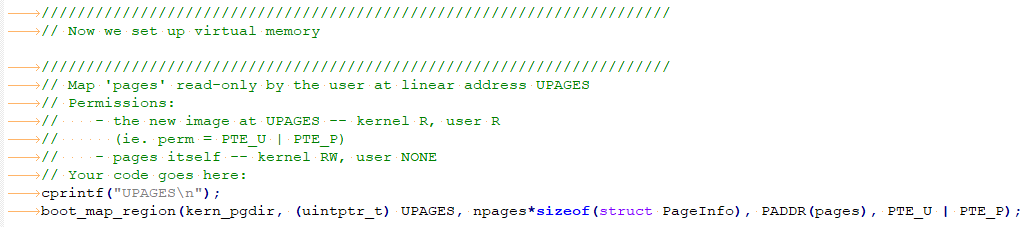
\includegraphics[width=0.8\linewidth]{figure/mem_init_changed1}
\end{figure}


Then there is the memory stack, the kernel stack ( 0xefff8000 \~ 0xf0000000) 32kB
Bootstrap represents the lowest address of the stack. Since the stack grows to the lower address, it is actually the top of the stack. We will map the address space in [KSTACKTOP-KSTKSIZE, KSTACKTOP)
The modified code is shown in the figure
\begin{figure}[H]
\centering
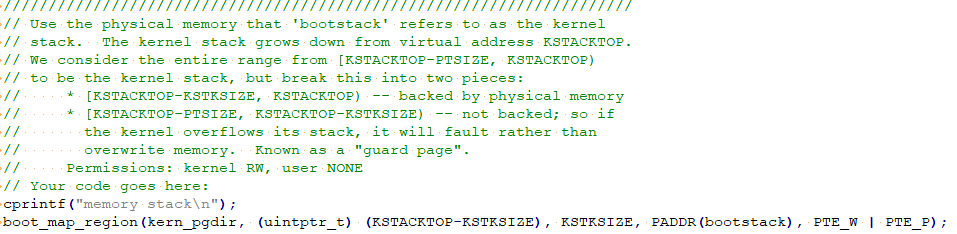
\includegraphics[width=0.8\linewidth]{figure/mem_init_changed2}
\end{figure}


Finally, the kernel part, we will map the kernel ( 0xf0000000 \~ 0xffffffff ) 256MB
The modified code is shown in the figure
\begin{figure}[H]
\centering
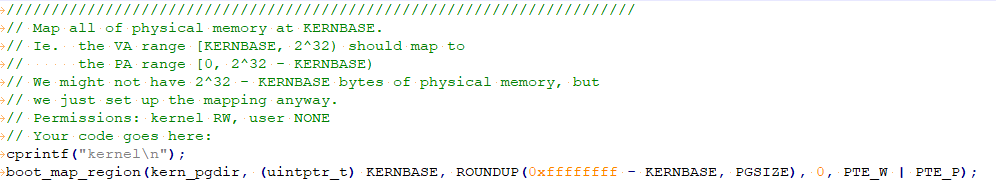
\includegraphics[width=0.8\linewidth]{figure/mem_init_changed3}
\end{figure}

As a result,  the code works successfully.

\begin{figure}[H]
\centering
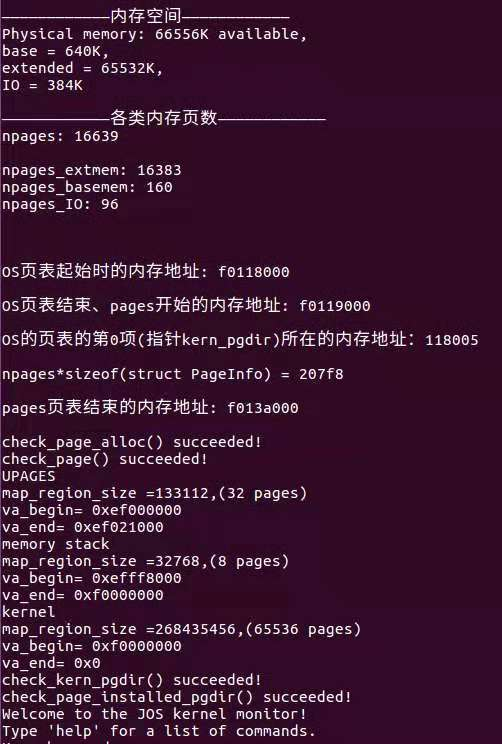
\includegraphics[width=0.8\linewidth]{figure/make_qemu}
\end{figure}

\begin{figure}[H]
\centering
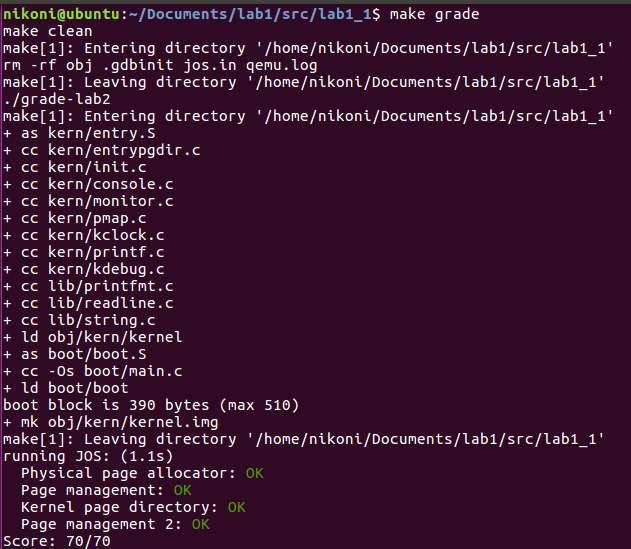
\includegraphics[width=0.8\linewidth]{figure/make_grade}
\end{figure}

\subsubsection{Question \Rmnum{4}}
\begin{flushleft}
1)\\
What entries (rows) in the page directory have been filled in at this point? What addresses do they map and where do they point? In other words, fill out this table as much as possible:
\begin{figure}[H]
\centering
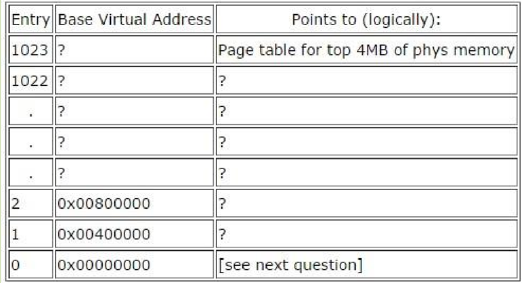
\includegraphics[width=0.8\linewidth]{figure/question4}
\end{figure}
\end{flushleft}
\begin{flushleft}
{\Large Answer}
\end{flushleft}
\begin{table}[H]
\centering
\begin{tabular}{ |p{150pt}<{\centering}|p{150pt}<{\centering}|p{150pt}<{\centering}| }
\hline				
Entry & Base Virtual Address &Points to(logically) \\ \hline 	
1023 & 0xffc00000 Points to(logically) & Page table for top 4MB of physical memory.This is the last address finding page table that the kernel can use.\\ \hline
1022 & 0xff800000 &Page table for 248MB--(252MB-1)physical memory \\ \hline 	
... & ... &Page table for physical memory \\ \hline
960 & 0xf0000000(KERNBASE) &static data 0--(4MB-1) physical memory \\ \hline
959 & 0xefc00000(VPT) &Page directory self (kernel RW).This is the first page table and it ’ s in the bottom of the physical memory. \\ \hline
958 & 0xef800000(ULIM) &Page table for kernel stack.It is mapped into the physical memory which is the same as bootstack.We only map the memory that the same as KSTACKSIZE.The rest memory that wasn’t mapped is used to avoid the overflow of the kernel stack. \\ \hline
957 & 0xef400000(UVPT) &Same as 959(user kernel R) \\ \hline
956 & 0xef00000(UPAGES) &Page table for structure pages[] \\ \hline
... & ... & NULL \\ \hline
2 & 0x00800000 & NULL \\ \hline
1 & 0x00400000 & NULL \\ \hline
0 & 0x00000000 & The start of the virtual memory .The same as 960(then turn to NULL)\\ \hline
\end{tabular}
\caption{Answer}
\end{table}

\begin{flushleft}
2)We have placed the kernel and user environment in the same address space. Why will user programs not be able to read or write the kernel's memory? What specific mechanisms protect the kernel memory?

{\Large Answer}
\end{flushleft}

User is not allowed to access kernel memory for safety reasons.
If user have the permission, bugs in user code may led to crash.
It is the paging mechanism that protects kernel address in JOS. If the flag bit PTE\_U is 0 in a page, that means user have no permission to read or write the page.

\begin{flushleft}
3)What is the maximum amount of physical memory that this operating system can support? Why?

{\Large Answer}
\end{flushleft}
\begin{figure}[H]
\centering
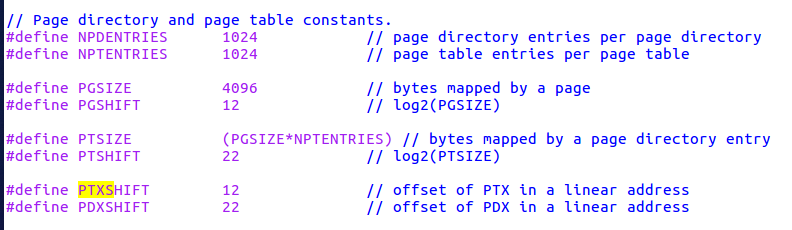
\includegraphics[width=0.8\linewidth]{figure/question4_3_1}
\caption{PTSIZE}
\end{figure}

\begin{figure}[H]
\centering
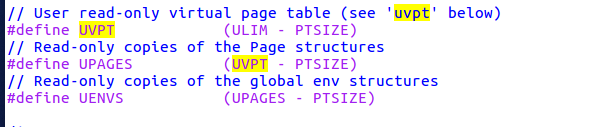
\includegraphics[width=0.8\linewidth]{figure/question4_3_2}
\caption{UPAGES}
\end{figure}

\begin{figure}[H]
\centering
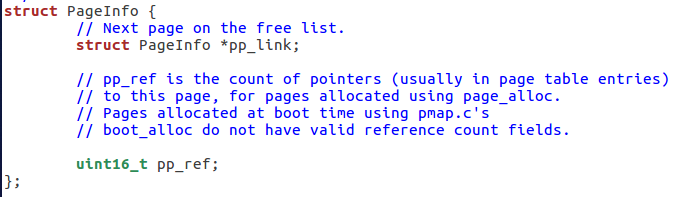
\includegraphics[width=0.8\linewidth]{figure/question4_3_3}
\caption{Page}
\end{figure}

2GB.

Pages use up to 4MB space, and each PageInfo use 8Byte. 4M / 8 * 4kB=2GB (4kB per page).


\begin{flushleft}
4)How much space overhead is there for managing memory, if we actually had the maximum amount of physical memory? How is this overhead broken down?

{\Large Answer}
\end{flushleft}

The total overhead to manage maxium amount of physical memory is:

  786432 bytes (struct Pages [1])

  4096 bytes (one page directory [2])

  262144 bytes (64 page tables [3])

  ------------

  1052672 bytes (~1MB)

  The only way I can see to reduce that amount is to use 4MB pages, this
  would reduce the struct Page allocations to 768 bytes and no need to
  allocate page tables.

  On the hand, the greater the granularity the greater the amount of
  unused chunks we'll have on the allocated pages which means we'll
  spend memory...

  [1] struct Page overhead was calculated this way
  256 * 1024 * 1024 / 4096 * 12
  256MB Page size size of struct Page

  [2] Page directory is 4096 bytes long by definition

  [3] Page table overhead was calculated this way

  (256 * 1024 * 1024 / (4096 * 1024)) * 4096
  256MB PG maps 4MB PG size
\clearpage
